\documentclass[10pt,aspectratio=169]{beamer}
\usetheme{Madrid}

%%──────────────────────────── COLORS ────────────────────────────────
\definecolor{mblue}{RGB}{22,88,158}
\definecolor{mlblue}{RGB}{210,228,248}
\definecolor{mred}{RGB}{185,50,40}
\definecolor{mgreen}{RGB}{30,150,80}
\definecolor{morange}{RGB}{200,100,0}

\setbeamercolor{palette primary}{bg=mblue,fg=white}
\setbeamercolor{palette secondary}{bg=mblue!78,fg=white}
\setbeamercolor{palette tertiary}{bg=mblue!55,fg=white}
\setbeamercolor{palette quaternary}{bg=mblue!30,fg=white}
\setbeamercolor{structure}{fg=mblue}
\setbeamercolor{section in toc}{fg=mblue}
\setbeamercolor{background canvas}{bg=white}
\setbeamercolor{frametitle}{bg=mblue,fg=white}
\setbeamercolor{block title}{bg=mblue,fg=white}
\setbeamercolor{block body}{bg=mlblue!50,fg=black}
\setbeamercolor{block title alerted}{bg=mred,fg=white}
\setbeamercolor{block body alerted}{bg=mred!12,fg=black}
\setbeamercolor{block title example}{bg=mgreen,fg=white}
\setbeamercolor{block body example}{bg=mgreen!10,fg=black}
\setbeamercolor{alerted text}{fg=mred}
\setbeamercolor{itemize item}{fg=mblue}
\setbeamercolor{enumerate item}{fg=mblue}

\setbeamerfont{frametitle}{series=\bfseries,size=\normalsize}
\setbeamerfont{block title}{series=\bfseries}
\setbeamerfont{title}{series=\bfseries,size=\Large}

%%──────────────────────────── PACKAGES ──────────────────────────────
\usepackage{amsmath,amssymb}
\usepackage{booktabs}
\usepackage{tikz}
\usepackage{pgfplots}
\pgfplotsset{compat=1.18}
\usetikzlibrary{arrows.meta,positioning,shapes.geometric,fit,backgrounds}
\usepackage{listings}
\usepackage{xcolor}
\usepackage{array}

\lstdefinestyle{pycode}{
  language=Python,
  basicstyle=\ttfamily\scriptsize,
  keywordstyle=\color{mblue}\bfseries,
  stringstyle=\color{mred!80},
  commentstyle=\itshape\color{gray},
  showstringspaces=false,
  breaklines=true,
  frame=single,
  rulecolor=\color{mblue!40},
  backgroundcolor=\color{mlblue!25},
  xleftmargin=4pt,xrightmargin=4pt,
}

%%──────────────────────────── METADATA ──────────────────────────────
\title[Data Drift --- Complete Course]{Data Drift: Complete Course}
\subtitle{Detection $\cdot$ Monitoring $\cdot$ Mitigation}
\author{ML Engineering Track}
\institute{Machine Learning in Production}
\date{\today}

%%═════════════════════════════════════════════════════════════════════
\begin{document}
%%═════════════════════════════════════════════════════════════════════

\begin{frame}
  \titlepage
\end{frame}

\begin{frame}{Agenda}
  \tableofcontents
\end{frame}

%%──────────────────────────────────────────────────────────────────
\section{The Problem}
%%──────────────────────────────────────────────────────────────────

\begin{frame}{Why Models Break in Production}
  \begin{columns}[T]
    \begin{column}{0.52\textwidth}
      \begin{alertblock}{Core Reality}
        A model trained on historical data is deployed into a \textbf{changing world}.\\[4pt]
        Accuracy silently drops --- no exceptions thrown, no alerts raised.
      \end{alertblock}
      \vspace{0.2cm}
      \textbf{Real-world triggers:}
      \begin{itemize}
        \item User behaviour and tastes evolve over time
        \item External shocks: COVID, regulations, market crashes
        \item Seasonal patterns not captured in training data
        \item Upstream data pipeline changes or schema breaks
        \item Population demographics shift
      \end{itemize}
    \end{column}
    \begin{column}{0.44\textwidth}
      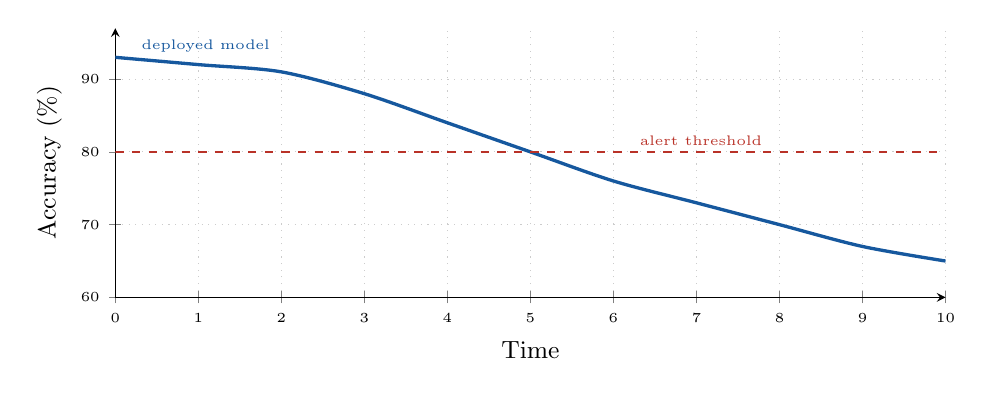
\begin{tikzpicture}
        \begin{axis}[
          width=\textwidth, height=5cm,
          xlabel={\small Time}, ylabel={\small Accuracy (\%)},
          xmin=0, xmax=10, ymin=60, ymax=97,
          grid=major, grid style={dotted,gray!40},
          axis lines=left,
          tick style={color=gray},
          tick label style={font=\tiny},
          label style={font=\small},
        ]
          \addplot[mblue, very thick, smooth] coordinates {
            (0,93)(1,92)(2,91)(3,88)(4,84)(5,80)(6,76)(7,73)(8,70)(9,67)(10,65)
          };
          \addplot[mred, dashed, thick] coordinates {(0,80)(10,80)};
          \node[font=\tiny, mred, anchor=west] at (axis cs:6.2,81.5) {alert threshold};
          \node[font=\tiny, mblue, anchor=west] at (axis cs:0.2,94.5) {deployed model};
        \end{axis}
      \end{tikzpicture}
    \end{column}
  \end{columns}
\end{frame}

\begin{frame}{Formal Setup}
  Let $P_{tr}(X,Y)$ = training joint distribution;\quad $P_{pr}(X,Y)$ = production joint distribution.
  \vspace{0.25cm}
  \begin{block}{No Drift Condition}
    \[ P_{tr}(X,Y) \;=\; P_{pr}(X,Y) \]
  \end{block}
  \vspace{0.25cm}
  The joint always factorises as:
  \[
    P(X,Y) \;=\; \underbrace{P(X)}_{\text{feature dist.}} \cdot \underbrace{P(Y|X)}_{\text{concept}}
              \;=\; \underbrace{P(Y)}_{\text{label prior}} \cdot \underbrace{P(X|Y)}_{\text{likelihood}}
  \]
  \begin{block}{Implication}
    Each factor can drift \emph{independently} --- this gives rise to the different \textbf{types} of drift, each requiring different detection and mitigation strategies.
  \end{block}
\end{frame}

%%──────────────────────────────────────────────────────────────────
\section{Taxonomy of Data Drift}
%%──────────────────────────────────────────────────────────────────

\begin{frame}{Three Fundamental Types}
  \begin{columns}[T]
    \begin{column}{0.32\textwidth}
      \begin{block}{1. Covariate Shift}
        \[ P_{tr}(X) \neq P_{pr}(X) \]
        \[ P(Y|X)\;\text{unchanged} \]
        \vspace{2pt}
        Input distribution changes. The label mapping holds but model extrapolates poorly.
      \end{block}
    \end{column}
    \begin{column}{0.32\textwidth}
      \begin{block}{2. Label / Prior Shift}
        \[ P_{tr}(Y) \neq P_{pr}(Y) \]
        \[ P(X|Y)\;\text{unchanged} \]
        \vspace{2pt}
        Class prior changes. Feature distribution given class stays stable.
      \end{block}
    \end{column}
    \begin{column}{0.32\textwidth}
      \begin{alertblock}{3. Concept Drift}
        \[ P_{tr}(Y|X) \neq P_{pr}(Y|X) \]
        \vspace{2pt}
        The \textbf{mapping} from inputs to outputs changes. Decision boundary itself shifts.\\[4pt]
        \textbf{Most dangerous type.}
      \end{alertblock}
    \end{column}
  \end{columns}
  \vspace{0.3cm}
  \begin{block}{Data Drift --- Umbrella Term}
    Any change in $P(X,Y)$ between training and production. Covariate shift is by far the most frequent type encountered in practice.
  \end{block}
\end{frame}

\begin{frame}{Concept Drift Subcategories}
  \begin{columns}[T]
    \begin{column}{0.48\textwidth}
      \textbf{Concept drift patterns:}
      \begin{itemize}
        \item \textbf{Sudden:} abrupt change at time $t_0$\\
              (new regulation, crisis event)
        \item \textbf{Gradual:} slow transition between two concepts
        \item \textbf{Incremental:} small stepwise accumulation over time
        \item \textbf{Recurring:} seasonal or cyclical (weekday vs weekend)
      \end{itemize}
      \vspace{0.2cm}
      \begin{alertblock}{Key Point}
        Concept drift \textbf{requires new labels + retraining}. Distribution matching alone cannot fix it.
      \end{alertblock}
    \end{column}
    \begin{column}{0.48\textwidth}
      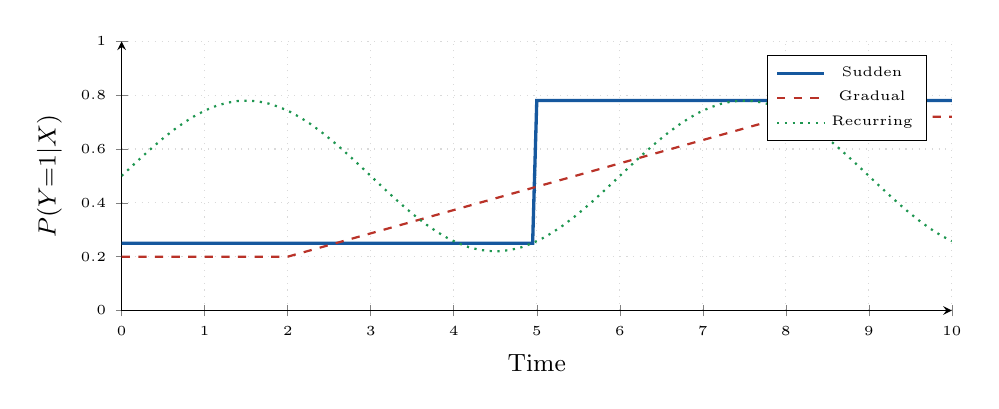
\begin{tikzpicture}
        \begin{axis}[
          width=\textwidth, height=5cm,
          xlabel={\small Time}, ylabel={\small $P(Y{=}1|X)$},
          xmin=0, xmax=10, ymin=0, ymax=1,
          grid=major, grid style={dotted,gray!30},
          axis lines=left,
          legend style={font=\tiny, at={(0.97,0.95)}, anchor=north east},
          tick label style={font=\tiny},
          label style={font=\small},
        ]
          \addplot[mblue, very thick] coordinates {
            (0,0.25)(4.95,0.25)(5,0.78)(10,0.78)
          };
          \addlegendentry{Sudden}
          \addplot[mred, thick, dashed] coordinates {
            (0,0.20)(2,0.20)(8,0.72)(10,0.72)
          };
          \addlegendentry{Gradual}
          \addplot[mgreen, thick, dotted, samples=80, domain=0:10]
            {0.5 + 0.28*sin(x*60)};
          \addlegendentry{Recurring}
        \end{axis}
      \end{tikzpicture}
    \end{column}
  \end{columns}
\end{frame}

\begin{frame}{Virtual vs Real Drift}
  \begin{columns}[T]
    \begin{column}{0.48\textwidth}
      \begin{block}{Virtual Drift $\equiv$ Covariate Shift}
        \begin{itemize}
          \item $P(X)$ changes;\; $P(Y|X)$ \textbf{unchanged}
          \item Model is theoretically still correct
          \item Performance drops due to extrapolation into low-density training regions
          \item Detectable from features alone --- \textbf{no labels needed}
          \item Can be partially corrected with \textbf{importance weighting}
        \end{itemize}
      \end{block}
    \end{column}
    \begin{column}{0.48\textwidth}
      \begin{alertblock}{Real Drift $\equiv$ Concept Drift}
        \begin{itemize}
          \item $P(Y|X)$ \textbf{changes}
          \item Model is fundamentally wrong
          \item Cannot be fixed without new labelled data
          \item Requires full or partial \textbf{retraining}
          \item Harder to detect: needs ground truth to confirm
        \end{itemize}
      \end{alertblock}
    \end{column}
  \end{columns}
  \vspace{0.3cm}
  \begin{block}{Production Reality}
    Labels arrive with a \textbf{delay} (hours to months). Monitor $P(X)$ and $P(\hat{Y})$ as proxies immediately; confirm concept drift only when labels arrive.
  \end{block}
\end{frame}

%%──────────────────────────────────────────────────────────────────
\section{Statistical Detection Methods}
%%──────────────────────────────────────────────────────────────────

\begin{frame}{Detection Framework}
  \textbf{General approach:} two-sample hypothesis test between a reference window and the current production window.
  \vspace{0.2cm}
  \begin{center}
  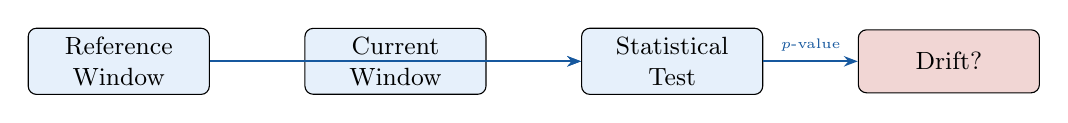
\begin{tikzpicture}[
    box/.style={draw, rounded corners=3pt, fill=mlblue!55, minimum width=2.3cm,
                minimum height=0.8cm, font=\small, align=center},
    arr/.style={-{Stealth[length=5pt]}, mblue, thick},
  ]
    \node[box] (ref)  {Reference\\Window};
    \node[box, right=1.2cm of ref]  (cur)  {Current\\Window};
    \node[box, right=1.2cm of cur]  (test) {Statistical\\Test};
    \node[box, right=1.2cm of test, fill=mred!20] (dec)  {Drift?};
    \draw[arr] (ref)  -- (test);
    \draw[arr] (cur)  -- (test);
    \draw[arr] (test) -- node[above,font=\tiny]{$p$-value} (dec);
  \end{tikzpicture}
  \end{center}
  \vspace{0.2cm}
  \begin{itemize}
    \item $H_0$: Reference and current distributions are \textbf{identical}
    \item $H_1$: Distributions \textbf{differ}
    \item Reject $H_0$ if $p\text{-value} < \alpha$ \quad (standard: $\alpha = 0.05$)
  \end{itemize}
  \vspace{0.1cm}
  \begin{alertblock}{Multiple Testing Problem}
    Testing $d$ features at once inflates false positive rate. Use \textbf{Bonferroni}: $\alpha' = \alpha/d$, or Benjamini-Hochberg for FDR control.
  \end{alertblock}
\end{frame}

\begin{frame}[fragile]{Kolmogorov-Smirnov Test --- Continuous Features}
  \textbf{Use for:} Any continuous univariate feature: age, income, latency, prediction score\ldots
  \vspace{0.15cm}
  \begin{block}{KS Statistic}
    \[
      D_{\mathrm{KS}} \;=\; \sup_{x}\,\bigl|F_{\mathrm{ref}}(x) - F_{\mathrm{cur}}(x)\bigr|
    \]
    $F_{\mathrm{ref}},\,F_{\mathrm{cur}}$ are empirical CDFs of the reference and current samples.
  \end{block}
  \vspace{0.15cm}
  \begin{columns}[T]
    \begin{column}{0.48\textwidth}
      \textbf{Properties:}
      \begin{itemize}
        \item Non-parametric --- no distribution assumption
        \item Sensitive to location, scale, and shape shifts
        \item $D_{\mathrm{KS}} \in [0,1]$; higher $\Rightarrow$ more drift
        \item Asymptotic $p$-value available in \texttt{scipy}
        \item Apply \textbf{per feature} --- univariate only
      \end{itemize}
    \end{column}
    \begin{column}{0.48\textwidth}
      \begin{exampleblock}{Python}
        \begin{lstlisting}[style=pycode]
from scipy.stats import ks_2samp

stat, pval = ks_2samp(
    ref_df['feature'],
    cur_df['feature']
)
if pval < 0.05:
    print("Drift detected!")
        \end{lstlisting}
      \end{exampleblock}
    \end{column}
  \end{columns}
\end{frame}

\begin{frame}{Population Stability Index (PSI)}
  \textbf{Use for:} Feature and model score monitoring (standard in credit risk)
  \vspace{0.15cm}
  \begin{block}{PSI Formula}
    \[
      \mathrm{PSI} \;=\; \sum_{i=1}^{k}\!\left(P_i^{\mathrm{cur}} - P_i^{\mathrm{ref}}\right)\ln\!\left(\frac{P_i^{\mathrm{cur}}}{P_i^{\mathrm{ref}}}\right)
    \]
    Bin the feature into $k{=}10$ equal-frequency bins derived from the reference distribution.
  \end{block}
  \vspace{0.2cm}
  \begin{center}
  \renewcommand{\arraystretch}{1.2}
  \begin{tabular}{@{}cll@{}}
    \toprule
    \textbf{PSI Value} & \textbf{Interpretation} & \textbf{Action} \\
    \midrule
    $< 0.10$      & \textcolor{mgreen}{No significant change}  & Continue monitoring \\
    $0.10 - 0.20$ & \textcolor{morange}{Slight shift detected} & Investigate root cause \\
    $> 0.20$      & \textcolor{mred}{Significant drift}        & Alert $+$ retrain \\
    \bottomrule
  \end{tabular}
  \end{center}
  \vspace{0.1cm}
  \textbf{Note:} Add $\varepsilon = 10^{-4}$ to empty buckets to avoid $\ln(0)$.
\end{frame}

\begin{frame}[fragile]{Chi-Squared Test --- Categorical Features}
  \textbf{Use for:} Any categorical feature: country, device type, product category\ldots
  \vspace{0.15cm}
  \begin{block}{Chi-Squared Statistic}
    \[
      \chi^2 \;=\; \sum_{i=1}^{k}\frac{(O_i - E_i)^2}{E_i}, \qquad \mathrm{df} = k-1
    \]
    $O_i$ = observed counts (current);\quad $E_i$ = expected counts (reference, scaled to $n_{\mathrm{cur}}$).
  \end{block}
  \vspace{0.15cm}
  \begin{columns}[T]
    \begin{column}{0.5\textwidth}
      \textbf{Requirements and caveats:}
      \begin{itemize}
        \item $E_i \geq 5$ per cell --- merge rare categories
        \item New categories in production not in reference $\Rightarrow$ always treat as drift
        \item Not order-sensitive (use KS for ordinals)
      \end{itemize}
    \end{column}
    \begin{column}{0.46\textwidth}
      \begin{exampleblock}{Python}
        \begin{lstlisting}[style=pycode]
from scipy.stats import chi2_contingency
import numpy as np

# ref_counts, cur_counts are arrays
# of per-category frequencies
obs = np.array([ref_counts,
                cur_counts])
chi2, pval, dof, _ = \
    chi2_contingency(obs)
        \end{lstlisting}
      \end{exampleblock}
    \end{column}
  \end{columns}
\end{frame}

\begin{frame}{Maximum Mean Discrepancy (MMD) --- Multivariate}
  \textbf{Use for:} High-dimensional data, embeddings (NLP, CV), correlated features
  \vspace{0.15cm}
  \begin{block}{MMD (kernel two-sample statistic)}
    \[
      \mathrm{MMD}^2(P,Q) \;=\;
        \mathbb{E}_{x,x'\sim P}[k(x,x')]
        \;-\; 2\,\mathbb{E}_{\substack{x\sim P \\ y\sim Q}}[k(x,y)]
        \;+\; \mathbb{E}_{y,y'\sim Q}[k(y,y')]
    \]
    Common kernel: RBF $\;k(x,y)=\exp\!\left(-\|x-y\|^2/2\sigma^2\right)$
  \end{block}
  \vspace{0.2cm}
  \textbf{Key properties:}
  \begin{itemize}
    \item $\mathrm{MMD}^2 = 0 \;\Leftrightarrow\; P = Q$ in a Reproducing Kernel Hilbert Space
    \item Captures inter-feature correlations --- univariate tests cannot do this
    \item Significance via \textbf{permutation test} (shuffle labels, recompute)
    \item $O(n^2)$ cost --- use random Fourier features for large datasets
    \item Implemented in \textbf{Alibi Detect} as \texttt{MMDDrift}
  \end{itemize}
\end{frame}

\begin{frame}[fragile]{ADWIN --- Adaptive Windowing for Streaming}
  \textbf{Use for:} Real-time drift detection in streaming pipelines (Kafka, Flink)
  \vspace{0.15cm}
  \begin{block}{Algorithm}
    Maintain a window $W$ of recent observations. Continuously search for cut-point $t$ such that:
    \[
      \bigl|\hat{\mu}_{W_0} - \hat{\mu}_{W_1}\bigr| \;\geq\; \varepsilon_{\mathrm{cut}}
    \]
    If found $\Rightarrow$ drift detected; drop older sub-window $W_0$ and shrink $W$.
  \end{block}
  \vspace{0.15cm}
  \begin{columns}[T]
    \begin{column}{0.54\textwidth}
      \textbf{Properties:}
      \begin{itemize}
        \item Window size adapts \textbf{automatically} --- no tuning
        \item Linear time $O(|W|)$ per incoming sample
        \item Apply to any 1D statistic: accuracy, feature mean, error rate
        \item Native in \textbf{River} and \textbf{scikit-multiflow}
      \end{itemize}
    \end{column}
    \begin{column}{0.42\textwidth}
      \begin{exampleblock}{Python (River)}
        \begin{lstlisting}[style=pycode]
from river import drift

detector = drift.ADWIN()
for x in data_stream:
    detector.update(x)
    if detector.drift_detected:
        retrain()
        \end{lstlisting}
      \end{exampleblock}
    \end{column}
  \end{columns}
\end{frame}

\begin{frame}{Detection Method Cheatsheet}
  \begin{center}
  \renewcommand{\arraystretch}{1.3}
  \begin{tabular}{@{}lccccc@{}}
    \toprule
    \textbf{Method}  & \textbf{Feature Type}  & \textbf{Univar.}
                     & \textbf{Multivar.}     & \textbf{Streaming} & \textbf{Complexity} \\
    \midrule
    KS Test          & Continuous      & \textcolor{mgreen}{\checkmark} & $\times$ & $\times$ & $O(n\log n)$ \\
    PSI              & Cont.\ / Ord.\  & \textcolor{mgreen}{\checkmark} & $\times$ & $\times$ & $O(n)$ \\
    Chi-Squared      & Categorical     & \textcolor{mgreen}{\checkmark} & $\times$ & $\times$ & $O(k)$ \\
    MMD              & Any             & \textcolor{mgreen}{\checkmark} & \textcolor{mgreen}{\checkmark} & $\times$ & $O(n^2)$ \\
    ADWIN            & Any (1D stat)   & \textcolor{mgreen}{\checkmark} & $\times$ & \textcolor{mgreen}{\checkmark} & $O(n)$ \\
    \bottomrule
  \end{tabular}
  \end{center}
  \vspace{0.25cm}
  \begin{block}{Decision Rule}
    \begin{itemize}
      \item Batch $+$ tabular $\;\to\;$ KS/PSI (continuous), Chi-Squared (categorical)
      \item Batch $+$ embeddings/images $\;\to\;$ MMD
      \item Streaming $\;\to\;$ ADWIN on key 1D metrics
    \end{itemize}
  \end{block}
\end{frame}

%%──────────────────────────────────────────────────────────────────
\section{Monitoring in Production}
%%──────────────────────────────────────────────────────────────────

\begin{frame}{What to Monitor}
  \begin{columns}[T]
    \begin{column}{0.48\textwidth}
      \begin{block}{Data-Level --- Leading Indicators}
        Available \textbf{immediately}, no labels needed:
        \begin{itemize}
          \item Feature distributions $P(X_j)$ per feature
          \item Missing value / null rates per column
          \item Feature correlation matrix shifts
          \item Prediction score distribution $P(\hat{Y})$
          \item Embedding drift (PCA / UMAP position)
        \end{itemize}
      \end{block}
    \end{column}
    \begin{column}{0.48\textwidth}
      \begin{alertblock}{Performance-Level --- Lagging Indicators}
        Require \textbf{ground-truth labels} --- often delayed:
        \begin{itemize}
          \item Accuracy, AUC-ROC, F1, RMSE
          \item Calibration (predicted vs.\ actual probability)
          \item Business KPIs (click-through, conversion rate)
          \item Human auditor or annotation feedback
        \end{itemize}
      \end{alertblock}
    \end{column}
  \end{columns}
  \vspace{0.3cm}
  \begin{block}{Label-Free Performance Estimation}
    \textbf{NannyML CBPE} (Confidence-Based Performance Estimation): estimates AUC from prediction confidence scores alone --- useful during the labelling delay window.
  \end{block}
\end{frame}

\begin{frame}{Windowing Strategies}
  \begin{columns}[T]
    \begin{column}{0.48\textwidth}
      \begin{block}{Reference vs Current}
        \begin{itemize}
          \item Fixed reference $=$ versioned training set
          \item Each production batch compared against it
          \item Simple; catches cumulative long-term drift
          \item Risk: reference itself becomes stale
        \end{itemize}
      \end{block}
      \vspace{0.2cm}
      \begin{block}{Sliding Window}
        \begin{itemize}
          \item Compare consecutive time windows
          \item No fixed anchor
          \item Better for detecting sudden, local drift
          \item May miss slow gradual drift vs.\ baseline
        \end{itemize}
      \end{block}
    \end{column}
    \begin{column}{0.48\textwidth}
      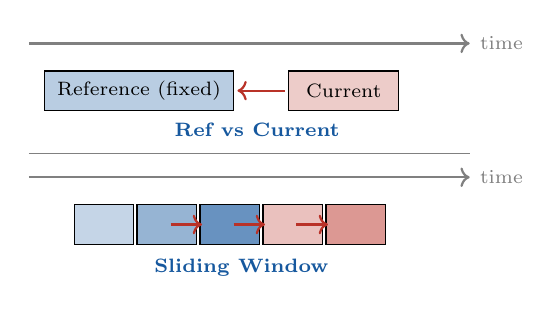
\begin{tikzpicture}
        \draw[->, gray, thick] (-0.2, 4.2) -- (5.4, 4.2)
          node[right, font=\scriptsize]{time};
        % Ref vs Current
        \node[draw, fill=mblue!30, minimum width=2.4cm, minimum height=0.5cm,
              font=\scriptsize, align=center] at (1.2, 3.6) {Reference (fixed)};
        \node[draw, fill=mred!25, minimum width=1.4cm, minimum height=0.5cm,
              font=\scriptsize, align=center] at (3.8, 3.6) {Current};
        \draw[mred,->,thick] (3.05,3.6) -- (2.45,3.6);
        \node[font=\scriptsize\bfseries, mblue] at (2.7, 3.1) {Ref vs Current};

        \draw[gray, thin] (-0.2, 2.8) -- (5.4, 2.8);
        \draw[->, gray, thick] (-0.2, 2.5) -- (5.4, 2.5)
          node[right, font=\scriptsize]{time};
        % Sliding windows - 5 boxes
        \node[draw, fill=mblue!25, minimum width=0.75cm, minimum height=0.5cm]
          at (0.75, 1.9) {};
        \node[draw, fill=mblue!45, minimum width=0.75cm, minimum height=0.5cm]
          at (1.55, 1.9) {};
        \node[draw, fill=mblue!65, minimum width=0.75cm, minimum height=0.5cm]
          at (2.35, 1.9) {};
        \node[draw, fill=mred!30, minimum width=0.75cm, minimum height=0.5cm]
          at (3.15, 1.9) {};
        \node[draw, fill=mred!50, minimum width=0.75cm, minimum height=0.5cm]
          at (3.95, 1.9) {};
        \draw[mred,->,thick] (1.6,1.9) -- (2.0,1.9);
        \draw[mred,->,thick] (2.4,1.9) -- (2.8,1.9);
        \draw[mred,->,thick] (3.2,1.9) -- (3.6,1.9);
        \node[font=\scriptsize\bfseries, mblue] at (2.5, 1.35) {Sliding Window};
      \end{tikzpicture}
    \end{column}
  \end{columns}
\end{frame}

\begin{frame}{Monitoring Pipeline Architecture}
  \begin{center}
  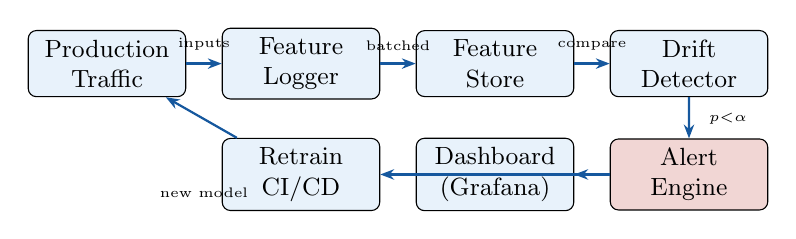
\begin{tikzpicture}[scale=0.88,
    box/.style={draw, rounded corners=3pt, fill=mlblue!50, minimum width=2cm,
                minimum height=0.75cm, font=\small, align=center},
    alert/.style={draw, rounded corners=3pt, fill=mred!20, minimum width=2cm,
                  minimum height=0.75cm, font=\small, align=center},
    arr/.style={-{Stealth[length=5pt]}, mblue, thick},
  ]
    \node[box]   (prod)  at (0,0)     {Production\\Traffic};
    \node[box]   (log)   at (2.8,0)   {Feature\\Logger};
    \node[box]   (store) at (5.6,0)   {Feature\\Store};
    \node[box]   (drift) at (8.4,0)   {Drift\\Detector};
    \node[alert] (al)    at (8.4,-1.6){Alert\\Engine};
    \node[box]   (dash)  at (5.6,-1.6){Dashboard\\(Grafana)};
    \node[box]   (ret)   at (2.8,-1.6){Retrain\\CI/CD};

    \draw[arr] (prod)  -- (log);
    \draw[arr] (log)   -- (store);
    \draw[arr] (store) -- (drift);
    \draw[arr] (drift) -- (al);
    \draw[arr] (al)    -- (dash);
    \draw[arr] (al)    -- (ret);
    \draw[arr] (ret)   -- (prod);

    \node[font=\tiny, above] at (1.4, 0.05)   {inputs};
    \node[font=\tiny, above] at (4.2, 0.05)   {batched};
    \node[font=\tiny, above] at (7.0, 0.05)   {compare};
    \node[font=\tiny, right] at (8.55,-0.8)   {$p{<}\alpha$};
    \node[font=\tiny, below] at (1.4,-1.65)   {new model};
  \end{tikzpicture}
  \end{center}
  \vspace{0.15cm}
  \begin{itemize}
    \item \textbf{Log} all inputs, predictions, and latencies with timestamps
    \item \textbf{Check} on schedule (hourly/daily) or trigger by incoming volume
    \item \textbf{Alert} via Slack / PagerDuty / custom webhook on drift signal
    \item \textbf{Retrain} automatically: drift signal $\to$ CI/CD trigger $\to$ shadow model $\to$ swap
  \end{itemize}
\end{frame}

%%──────────────────────────────────────────────────────────────────
\section{Tools \& Frameworks}
%%──────────────────────────────────────────────────────────────────

\begin{frame}{Production-Ready Tools}
  \begin{center}
  \renewcommand{\arraystretch}{1.25}
  \begin{tabular}{@{}p{2.6cm}p{2.8cm}p{6.2cm}@{}}
    \toprule
    \textbf{Tool}         & \textbf{Type}    & \textbf{Key Strengths} \\
    \midrule
    \textbf{Evidently AI} & Open-source      & 50+ metrics, HTML/JSON reports, MLflow integration \\
    \textbf{Alibi Detect} & Open-source      & MMD, LSDD, classifier-based; PyTorch/TF backends \\
    \textbf{NannyML}      & Open-source      & Label-free perf estimation (CBPE); handles label delay \\
    \textbf{WhyLabs}      & SaaS             & Always-on profiling, LLM monitoring, data sketches \\
    \textbf{Arize AI}     & SaaS             & Embedding drift, SHAP explanations, model observatory \\
    \textbf{Seldon Alibi} & K8s-native       & Drift detector as microservice sidecar in production \\
    \bottomrule
  \end{tabular}
  \end{center}
  \vspace{0.2cm}
  \begin{block}{Quick Recommendation}
    Start with \textbf{Evidently AI} for batch tabular systems.
    Add \textbf{Alibi Detect} for embeddings or multivariate drift.
    Use \textbf{NannyML} when label delay exceeds your acceptable blindspot.
  \end{block}
\end{frame}

\begin{frame}[fragile]{Evidently AI --- Practical Example}
  \begin{lstlisting}[style=pycode]
import pandas as pd
from evidently.report import Report
from evidently.metric_preset import DataDriftPreset, DataQualityPreset

reference = pd.read_csv("train_features.csv")
current   = pd.read_csv("prod_week1.csv")

report = Report(metrics=[
    DataDriftPreset(),    # KS for continuous, Chi2 for categorical -- auto-selected
    DataQualityPreset(),  # nulls, out-of-range values, outliers
])
report.run(reference_data=reference, current_data=current)
report.save_html("drift_report.html")   # rich interactive report

# Programmatic access
result       = report.as_dict()
drift_share  = result["metrics"][0]["result"]["share_of_drifted_columns"]
drifted_cols = [
    col for col, v in
    result["metrics"][0]["result"]["drift_by_columns"].items()
    if v["drift_detected"]
]
print(f"{drift_share:.0%} of features drifted: {drifted_cols}")
  \end{lstlisting}
\end{frame}

\begin{frame}[fragile]{Alibi Detect --- MMD for Embeddings}
  \begin{lstlisting}[style=pycode]
import numpy as np
from alibi_detect.cd import MMDDrift

X_ref  = np.load("X_train_embeddings.npy")  # shape: (n_ref, d)
X_prod = np.load("X_prod_embeddings.npy")   # shape: (n_cur, d)

# RBF kernel; permutation test for p-value; 200 permutations
detector = MMDDrift(X_ref, backend='pytorch', p_val=0.05, n_permutations=200)

result = detector.predict(X_prod)
print("Drift detected :", result['data']['is_drift'])   # True / False
print("p-value        :", result['data']['p_val'])
print("MMD^2          :", result['data']['distance'])
  \end{lstlisting}
  \vspace{0.1cm}
  \begin{block}{When to prefer Alibi Detect over Evidently}
    Sentence embeddings, image feature vectors, tabular data with strong inter-feature correlations --- any case where per-feature tests miss the joint distribution structure.
  \end{block}
\end{frame}

%%──────────────────────────────────────────────────────────────────
\section{Mitigation Strategies}
%%──────────────────────────────────────────────────────────────────

\begin{frame}{Mitigation Options}
  \begin{columns}[T]
    \begin{column}{0.48\textwidth}
      \begin{block}{1. Importance Weighting}
        Reweight training samples to match production:\\[4pt]
        \[
          w(x) \;=\; \frac{P_{pr}(x)}{P_{tr}(x)}
        \]
        \begin{itemize}
          \item No retraining on new data required
          \item Works for \textbf{covariate shift only}
          \item Estimation: KMM, KLIEP, or classifier-based\\
                (train binary classifier train vs prod; use predicted probabilities as weights)
        \end{itemize}
        \textbf{Fails} if $\mathrm{supp}(P_{pr}) \not\subseteq \mathrm{supp}(P_{tr})$.
      \end{block}
    \end{column}
    \begin{column}{0.48\textwidth}
      \begin{block}{2. Retraining}
        Retrain on recent labelled data:
        \begin{itemize}
          \item \textbf{Trigger:} scheduled / drift-signal / performance drop
          \item \textbf{Data:} sliding window of last $N$ days
          \item \textbf{Shadow model:} train in background, swap on improvement
          \item Handles both virtual and real drift
        \end{itemize}
      \end{block}
      \vspace{0.2cm}
      \begin{alertblock}{Check Pipeline First}
        Before retraining: verify the drift is not a \textbf{data pipeline bug} (schema change, null explosion, upstream ETL failure). Most production ``drift'' is actually a data bug.
      \end{alertblock}
    \end{column}
  \end{columns}
\end{frame}

\begin{frame}{Online \& Continual Learning}
  \textbf{For streaming or rapidly changing environments (low labelling cost):}
  \vspace{0.2cm}
  \begin{columns}[T]
    \begin{column}{0.48\textwidth}
      \begin{block}{Online Learning Algorithms}
        \begin{itemize}
          \item \textbf{SGD / Adam} on mini-batches from stream
          \item \textbf{FTRL} (Follow The Regularized Leader) --- ads, ranking systems
          \item \textbf{Hoeffding Trees} --- adaptive decision trees (\textbf{River} lib)
          \item \textbf{Passive-Aggressive} classifiers for fast adaptation
        \end{itemize}
      \end{block}
    \end{column}
    \begin{column}{0.48\textwidth}
      \begin{alertblock}{Catastrophic Forgetting}
        Learning new patterns erases old ones. Mitigations:
        \begin{itemize}
          \item \textbf{Experience Replay:} mix past samples into each batch
          \item \textbf{EWC} (Elastic Weight Consolidation): penalise changes to important weights
          \item \textbf{Progressive Nets:} freeze old columns, grow new ones
        \end{itemize}
      \end{alertblock}
    \end{column}
  \end{columns}
  \vspace{0.2cm}
  \begin{exampleblock}{Domain Adaptation}
    When some labelled target data is available: fine-tune on target domain, use adversarial domain adaptation (DANN), or pseudo-labelling on unlabelled production data.
  \end{exampleblock}
\end{frame}

%%──────────────────────────────────────────────────────────────────
\section{Summary \& Checklist}
%%──────────────────────────────────────────────────────────────────

\begin{frame}{Production Drift Checklist}
  \begin{columns}[T]
    \begin{column}{0.48\textwidth}
      \textbf{Before Deployment:}
      \begin{itemize}
        \item[$\square$] Version and store the reference dataset
        \item[$\square$] Choose detection method per feature type
        \item[$\square$] Set significance thresholds ($\alpha$, PSI cuts)
        \item[$\square$] Instrument feature logging in serving code
        \item[$\square$] Define retraining trigger criteria
      \end{itemize}
      \vspace{0.2cm}
      \textbf{After Deployment:}
      \begin{itemize}
        \item[$\square$] Schedule drift checks (hourly or daily)
        \item[$\square$] Monitor $P(\hat{Y})$ and critical features
        \item[$\square$] Set up alerting (Slack / PagerDuty)
        \item[$\square$] Track ground-truth performance when labels arrive
      \end{itemize}
    \end{column}
    \begin{column}{0.48\textwidth}
      \textbf{When Drift is Detected:}
      \begin{itemize}
        \item[$\square$] Identify which features drifted
        \item[$\square$] Classify: virtual (covariate) or real (concept)?
        \item[$\square$] Rule out upstream pipeline bugs first
        \item[$\square$] Apply appropriate mitigation strategy
        \item[$\square$] A/B test new model before full rollout
        \item[$\square$] Document the incident
      \end{itemize}
      \vspace{0.2cm}
      \begin{alertblock}{Golden Rule}
        \textbf{Always check your data pipeline before assuming model drift.} Schema changes and ETL failures cause the majority of production ``drift'' incidents.
      \end{alertblock}
    \end{column}
  \end{columns}
\end{frame}

\begin{frame}{The Full Picture}
  \begin{center}
  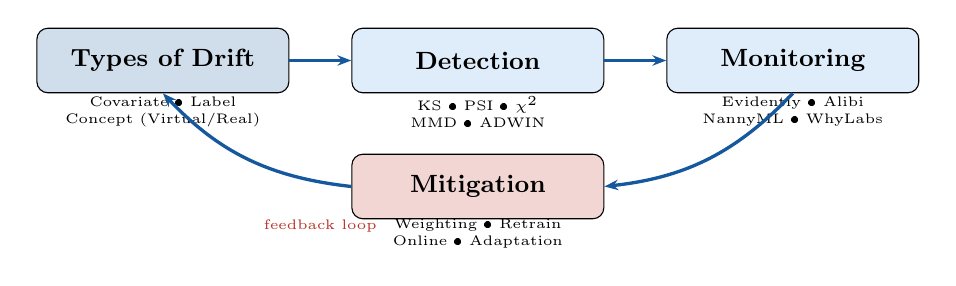
\begin{tikzpicture}[
    box/.style={draw, rounded corners=4pt, minimum width=3.2cm, minimum height=0.82cm,
                font=\small\bfseries, align=center},
    sub/.style={font=\tiny, text width=3.2cm, align=center},
    arr/.style={-{Stealth[length=5pt]}, mblue, very thick},
  ]
    \node[box, fill=mblue!20]  (T) at (0,3)    {Types of Drift};
    \node[box, fill=mlblue!70] (D) at (4,3)    {Detection};
    \node[box, fill=mlblue!70] (M) at (8,3)    {Monitoring};
    \node[box, fill=mred!20]   (R) at (4,1.4)  {Mitigation};

    \node[sub] at (0,2.35)  {Covariate \textbullet\ Label\\Concept (Virtual/Real)};
    \node[sub] at (4,2.35)  {KS \textbullet\ PSI \textbullet\ $\chi^2$\\MMD \textbullet\ ADWIN};
    \node[sub] at (8,2.35)  {Evidently \textbullet\ Alibi\\NannyML \textbullet\ WhyLabs};
    \node[sub] at (4,0.8)   {Weighting \textbullet\ Retrain\\Online \textbullet\ Adaptation};

    \draw[arr] (T) -- (D);
    \draw[arr] (D) -- (M);
    \draw[arr] (M.south) to[bend left=20] (R.east);
    \draw[arr] (R.west) to[bend left=20] (T.south);
    \node[font=\tiny, mred] at (2.0, 0.9) {feedback loop};
  \end{tikzpicture}
  \end{center}
  \vspace{0.15cm}
  \begin{block}{4 Things to Remember}
    \begin{enumerate}
      \item Data drift is \textbf{inevitable} --- build monitoring from day one, not after the model degrades
      \item Monitor $P(X)$ immediately as proxy; confirm concept drift only when labels arrive
      \item Match detection method to data type; apply multiple testing correction for many features
      \item Automate the full loop: drift signal $\to$ retrain trigger $\to$ shadow model $\to$ A/B $\to$ swap
    \end{enumerate}
  \end{block}
\end{frame}

\end{document}
